\documentclass[11pt]{article}
\ifdefined\pdfinfoomitdate\pdfinfoomitdate=1\fi
\ifdefined\pdftrailerid\pdftrailerid{}\fi
\ifdefined\pdfsuppressptexinfo\pdfsuppressptexinfo=15\fi
\usepackage[T1]{fontenc}
\usepackage{lmodern}
\ifdefined\pdfglyphtounicode
  \pdfgentounicode=1
  \pdfglyphtounicode{tfm:lmex10/parenleftbig}{0028}
  \pdfglyphtounicode{tfm:lmex10/parenrightbig}{0029}
  \pdfglyphtounicode{tfm:lmex10/bracketleftbig}{005B}
  \pdfglyphtounicode{tfm:lmex10/bracketrightbig}{005D}
  \pdfglyphtounicode{tfm:lmex10/parenleftBig}{0028}
  \pdfglyphtounicode{tfm:lmex10/parenrightBig}{0029}
  \pdfglyphtounicode{tfm:lmex10/parenleftbigg}{0028}
  \pdfglyphtounicode{tfm:lmex10/parenrightbigg}{0029}
  \pdfglyphtounicode{tfm:lmex10/braceleftbigg}{007B}
  \pdfglyphtounicode{tfm:lmex10/bracerightbigg}{007D}
  \pdfglyphtounicode{tfm:lmex10/parenleftBigg}{0028}
  \pdfglyphtounicode{tfm:lmex10/parenrightBigg}{0029}
  \pdfglyphtounicode{tfm:lmex10/bracketleftBig}{005B}
  \pdfglyphtounicode{tfm:lmex10/bracketrightBig}{005D}
  \pdfglyphtounicode{tfm:lmex10/integraltext}{222B}
  \pdfglyphtounicode{tfm:lmex10/integraldisplay}{222B}
  \pdfglyphtounicode{tfm:lmex10/summationdisplay}{2211}
  \pdfglyphtounicode{tfm:lmex10/vextendsingle}{23D0}
  \pdfglyphtounicode{tfm:lmex10/bracelefttp}{23A7}
  \pdfglyphtounicode{tfm:lmex10/braceleftmid}{23A8}
  \pdfglyphtounicode{tfm:lmex10/braceleftbt}{23A9}
  \pdfglyphtounicode{tfm:lmsy10/mapsto}{007C}
  \pdfglyphtounicode{tfm:lmsy10/D}{1D49F}
  \pdfglyphtounicode{tfm:lmsy10/K}{1D4A6}
  \pdfglyphtounicode{tfm:msbm10/E}{1D53C}
  \pdfglyphtounicode{tfm:msbm10/P}{2119}
  \pdfglyphtounicode{tfm:msbm10/R}{211D}
  \pdfglyphtounicode{tfm:msbm10/S}{1D54A}
  \pdfglyphtounicode{tfm:lmmi10/mu}{03BC}
  \pdfglyphtounicode{tfm:rm-lmr10/Delta}{0394}
\fi
\usepackage[margin=1.08in]{geometry}
\usepackage{amsmath,amssymb,amsthm,mathtools}
\usepackage{microtype,graphicx,booktabs,enumitem,flafter}
\usepackage{xcolor,tikz}
\usetikzlibrary{arrows.meta,positioning,calc}
\usepackage{cite}
\usepackage{xurl}
\usepackage[hidelinks,breaklinks]{hyperref}
\hypersetup{
  pdftitle={The Subcritical Henon--Lane--Emden Conjecture},
  pdfauthor={OpenAI}
}
\newtheorem{theorem}{Theorem}[section]
\newtheorem{proposition}[theorem]{Proposition}
\newtheorem{lemma}[theorem]{Lemma}
\newtheorem{corollary}[theorem]{Corollary}
\theoremstyle{definition}
\newtheorem{definition}[theorem]{Definition}
\newtheorem{remark}[theorem]{Remark}
\newcommand{\R}{\mathbb R}
\newcommand{\dd}{\,\mathrm d}
\newcommand{\eps}{\varepsilon}
\newcommand{\Sph}{\mathbb S^{n-1}}
\numberwithin{equation}{section}
\setlist{itemsep=3pt,topsep=5pt}
\setlength{\emergencystretch}{2em}
\title{The Subcritical H\'enon--Lane--Emden Conjecture}
\author{OpenAI}
\date{September 24, 2026}
\begin{document}
\maketitle
\begin{abstract}
We prove the subcritical H\'enon--Lane--Emden conjecture: for every
dimension $n\ge2$, positive powers $p,q$, and real weights $A,B$, the
system has no strictly positive entire solution when
$(n+A)/(p+1)+(n+B)/(q+1)>n-2$. Solutions need only be continuous at
the origin and classical elsewhere, without a condition at infinity.
For \(n\ge3\) and \(A,B>-2\), combining this result with the radial
existence theorem of Bidaut-V\'eron and Giacomini proves Phan's
Conjecture~C in full: a positive radial entire solution exists whenever
the strict inequality fails.
\end{abstract}
\tableofcontents
\section{Introduction}\label{sec:introduction}

The H\'enon--Lane--Emden system is
\begin{equation}\label{eq:system}
 -\Delta u=|x|^A v^p,\qquad
 -\Delta v=|x|^B u^q
 \qquad\text{in }\R^n\setminus\{0\}.
\end{equation}
Its subcritical nonexistence conjecture asks whether the weighted
hyperbola alone rules out positive solutions, without symmetry or
conditions at infinity. The unweighted case \(A=B=0\) is the classical
Lane--Emden system.

The scalar subcritical Liouville theorem of Gidas and Spruck is a
starting point for this question~\cite{GidasSpruck1981}. For systems,
Mitidieri developed a Rellich identity and early nonexistence
regions~\cite{Mitidieri1993,Mitidieri1996}. Serrin and Zou proved the
unweighted three-dimensional assertion under a growth condition;
Pol\'a\v{c}ik, Quittner, and Souplet removed that condition, and
Souplet settled dimension four~\cite{SerrinZou1996,
PolacikQuittnerSouplet2007,Souplet2009}. Li, Li, and Wei obtained a
further unweighted nonexistence region for \(p,q\ge1\) in every dimension
\(n\ge5\)~\cite[Theorem~1.1]{LiLiWei2025}. Liouville theorems also serve
as inputs to rescaling arguments for a priori bounds and singularity
estimates~\cite{GidasSpruckBounds1981,PolacikQuittnerSouplet2007}.

For the weighted system, Bidaut-V\'eron and Giacomini identified the
critical hyperbola in the regular radial theory under admissible
weights~\cite{BidautVeronGiacomini2010}. Phan formulated the unrestricted
weighted question for \(A,B>-2\) as Conjecture~C and established
bounded, low-dimensional, and conditional cases~\cite{Phan}.
Fazly and Ghoussoub obtained bounded and stability-based results for
nonnegative weights~\cite{FazlyGhoussoub2014}; Li and Zhang subsequently
proved the weighted conjecture in dimension three without a boundedness
assumption~\cite{LiZhang2019}. Results in restricted exponent ranges
extend to dimensions four and five~\cite{Li2022}. More recently,
Huang and Zou stated the all-real-weight, origin-continuous assertion
as Conjecture~B and proved cases with stability, decay, or energy
hypotheses~\cite{HuangZou}. Xu and Luo obtained a higher-order weighted
theorem over the full exponent range for radial solutions subject to
regularity and growth conditions~\cite{XuLuo2026}. The full nonradial
question in higher dimensions is the subject of this paper.

\begin{theorem}\label{thm:main}
Let \(n\ge2\) be an integer, let \(p,q>0\), and let \(A,B\in\R\).
Suppose that
\begin{equation}\label{eq:subcritical}
 \frac{n+A}{p+1}+\frac{n+B}{q+1}>n-2.
\end{equation}
There are no functions
\[
 u,v\in C^2(\R^n\setminus\{0\})\cap C(\R^n),
 \qquad u(x)>0,\quad v(x)>0\quad(x\in\R^n),
\]
satisfying Equation~\eqref{eq:system} at every \(x\ne0\).
\end{theorem}

\begin{corollary}[Unweighted Lane--Emden conjecture]
\label{cor:lane-emden}
For every integer \(n\ge3\) and \(p,q>0\) satisfying
\[
 \frac{1}{p+1}+\frac{1}{q+1}>\frac{n-2}{n},
\]
there is no strictly positive \(C^2(\R^n)\) solution of
\[
 -\Delta u=v^p,\qquad -\Delta v=u^q\qquad\text{in }\R^n.
\]
\end{corollary}

In particular, positivity at the origin is part of the hypothesis,
but differentiability there is not. No radial symmetry, boundedness,
integrability, finite energy, stability, or growth or decay condition
at infinity is required.

Theorem~\ref{thm:main} resolves Huang and Zou's Conjecture~B positively
and yields Corollary~\ref{cor:lane-emden} by setting \(A=B=0\).
For \(n\ge3\) and \(A,B>-2\), its nonexistence conclusion joins the
radial existence theorem of Bidaut-V\'eron and
Giacomini~\cite[Theorem~1.4(i)]{BidautVeronGiacomini2010} to prove Phan's
Conjecture~C in full, including existence on the critical hyperbola.
Corollary~\ref{cor:phan-classification} records this derived classification.
The weak regularity at the origin is genuine: positivity and continuity,
rather than a prescribed order of vanishing or smoothness there, are all
that is assumed.

The weighted assertion cannot be inferred merely by applying the
unweighted assertion at the same exponents. For instance,
\(n=5\), \(p=q=4\), \(A=B=3\) satisfies
Equation~\eqref{eq:subcritical}, whereas
\(1/(p+1)+1/(q+1)=2/5<3/5\).
Likewise, the unweighted input in Phan's transfer argument must remain
within its actual scope; weighted subcriticality does not imply that
input~\cite{Phan}.

\paragraph{The weighted argument.}
Rellich--Pohozaev identities and spherical estimates have long been
central to system Liouville proofs~\cite{Mitidieri1993,Souplet2009,Phan}.
Chen and Li used Newtonian integral representations with moving planes
under integrability hypotheses~\cite{ChenLi2009}; Cheng and Huang later
formulated an energy-estimate criterion for the unweighted
conjecture~\cite{ChengHuang2019}. The passage from a uniform local
weighted-energy bound to nonexistence by origin-centered dilation also
appears in Li~\cite[Section~2]{Li2022}. Here a localized potential-kernel
virial identity and an energy-relative interval-pressure estimate supply
that bound throughout the subcritical range.

There are two difficulties in passing from unweighted source layers
to Equation~\eqref{eq:system}. Translations do not preserve the
equation, and an endpoint of a layer
\(\{|x|^B u(x)^q>t\}\) has value
\((t/|x|^B)^{1/q}\), not the constant \(t^{1/q}\).
We address both directly.

First, origin-centered dilations give uniform source masses and
truncated-potential bounds on a fixed ball. A compactly supported
virial identity then retains the exact spatial-weight coefficients.
Second, the interval comparison is applied with directions in a
small cap around the radial direction and with weights constant on
each retained interval. Retained intervals are short enough that
their endpoint weight variation is small. The discarded intervals
are controlled by polar integration of source masses and a
high/low layer decomposition.

All errors are arbitrarily small relative to a fixed localized
energy, up to a universal additive constant. No bound on that energy
is assumed in obtaining the error estimates. The weighted
subcritical gap then supplies such a bound, and dilation gives a
contradiction. This combination of spatially varying directional
cutoffs, intervalwise infima, and energy-relative layer errors is
the part of the method that may be useful for other weighted
potential systems. The elementary interval comparison itself is
reproved below.

\paragraph{Organization.}
Section~\ref{sec:preliminaries} treats the origin, the low-exponent
cases, and the potential estimates.
Section~\ref{sec:localization} proves the localized virial identity
and compares the two localized interaction marginals.
Section~\ref{sec:intervals} gives the geometric interval inequality.
Section~\ref{sec:pressure} proves its weighted pressure consequence,
including the needed layer-error bounds.
Section~\ref{sec:conclusion} completes the proof by scaling and derives
the existence--nonexistence classification from the radial theorem.

\section{Reductions and Newton potentials}\label{sec:preliminaries}

We begin with consequences of positivity that do not require the
subcritical inequality.  Throughout this section, a solution means a pair
\[
 u,v\in C^2(\R^n\setminus\{0\})\cap C(\R^n),\qquad u,v>0
 \quad\hbox{on }\R^n,
\]
where $n\ge2$, $p,q>0$, and $A,B\in\R$, satisfying
\[
 -\Delta u=|x|^A v^p,\qquad -\Delta v=|x|^B u^q
 \quad\hbox{on }\R^n\setminus\{0\}.
\]
We write $B_R(z)=\{x:|x-z|<R\}$ and $B_R=B_R(0)$.

\begin{lemma}[Origin reductions]\label{lem:reductions}
The existence of a solution implies $n\ge3$ and $A,B>-2$.
\end{lemma}

\begin{proof}
For a function $h$ continuous on each sphere about the origin, write
\[
 \overline h(r)=\frac1{|\Sph|}\int_{\Sph}h(r\theta)\,\dd\theta.
\]
Integration of the equations on annuli gives, for $r>0$,
\begin{equation}\label{eq:spherical-flux}
 \begin{split}
  \bigl(r^{n-1}\overline u'(r)\bigr)'
     &=-r^{n-1+A}\overline{v^p}(r),\\
  \bigl(r^{n-1}\overline v'(r)\bigr)'
     &=-r^{n-1+B}\overline{u^q}(r).
 \end{split}
\end{equation}
In particular, each flux on the left is strictly decreasing.  Its extended
limit as $r\downarrow0$ exists.  If that limit were nonzero or infinite,
the flux would have a fixed sign and absolute value bounded below by a
positive constant for all sufficiently small $r$.  Since
$\int_0^1 r^{1-n}\,\dd r=\infty$, integration would contradict boundedness
of the corresponding spherical mean at zero.  Thus both limits are zero,
and both fluxes are strictly negative for every $r>0$.

If $n=2$, then $r\overline u'(r)\le\overline u'(1)<0$ for $r\ge1$.
Consequently
$\overline u(r)\le\overline u(1)+\overline u'(1)\log r$, contradicting
positivity for large $r$.

Continuity and $v(0)>0$ give $v^p\ge c>0$ near zero.  Integrating the first
equation in \eqref{eq:spherical-flux} over $[r/2,r]$ and using the negative
flux at $r/2$, we obtain
\[
 -\overline u'(r)
 \ge c r^{1-n}\int_{r/2}^r s^{n-1+A}\,\dd s
 =c_A r^{1+A},\qquad c_A>0.
\]
The equality remains valid when $n+A=0$, with the corresponding constant
containing $\log2$.  If $A\le-2$, integrating this inequality towards
zero contradicts continuity of $u$ there.  Interchanging the two equations
proves $B>-2$.
\end{proof}

Henceforth assume $n\ge3$ and $A,B>-2$.  Define, off zero,
\begin{equation}\label{eq:sources-kernel}
 \begin{gathered}
 f(x)=|x|^B u(x)^q,\qquad g(x)=|x|^A v(x)^p,\\
 K(x)=c_n|x|^{2-n},\qquad c_n=\frac1{(n-2)|\Sph|}.
 \end{gathered}
\end{equation}
We set $f(0)=g(0)=0$, which has no effect on any integral.  All unspecified
integrals below are Lebesgue integrals.  A constant called \emph{universal}
may depend on $n,p,q,A,B$ and on explicitly indicated auxiliary parameters,
but not on the particular solution.  In contrast, constants denoted by
$C_{u,v}$ are allowed to depend on the solution.

\begin{lemma}[Distributional extension and potentials]\label{lem:potential}
For every solution with $n\ge3$ and $A,B>-2$, the sources $f,g$ belong to
$L^1_{\mathrm{loc}}(\R^n)$ and
\[
 -\Delta u=g,\qquad -\Delta v=f
 \quad\hbox{in distributions on }\R^n.
\]
The Newton potentials are finite everywhere and satisfy
\begin{equation}\label{eq:potential-lower}
 K*g\le u,\qquad K*f\le v \quad\hbox{on }\R^n.
\end{equation}
There are constants $c_u,c_v\ge0$ such that
\begin{equation}\label{eq:potential-constants}
 u=c_u+K*g,\qquad v=c_v+K*f
\end{equation}
almost everywhere on $\R^n$ and pointwise on $\R^n\setminus\{0\}$.
On the latter set the potentials are continuously differentiable, and
\begin{equation}\label{eq:potential-gradients}
 \begin{split}
 \nabla u(x)&=\int_{\R^n}\nabla K(x-y)g(y)\,\dd y,\\
 \nabla v(x)&=\int_{\R^n}\nabla K(x-y)f(y)\,\dd y,\\
 \nabla K(z)&=-(n-2)\frac{z}{|z|^2}K(z).
 \end{split}
\end{equation}
Both gradient integrals converge absolutely at every $x\ne0$.
\end{lemma}

\begin{proof}
Local boundedness of $u,v$ gives
$g(x)\le C_{u,v}|x|^A$ and $f(x)\le C_{u,v}|x|^B$ near zero.
Since $n+A,n+B>0$, both sources are locally integrable.  Let
$\varphi\in C_c^\infty(\R^n)$ and choose
$\xi\in C_c^\infty(\R^n)$ equal to one near zero.  Test the equation for
$u$ away from zero against
$\varphi(x)(1-\xi(x/\rho))$.  After expanding its Laplacian, the terms
involving first and second derivatives of $\xi(x/\rho)$ have absolute
values bounded respectively by $C_{u,v,\varphi,\xi}\rho^{n-1}$ and
$C_{u,v,\varphi,\xi}\rho^{n-2}$.  They tend to zero.  The remaining
terms pass to the limit by local integrability, proving the first
distributional equation.  The second follows in the same way.

Let $\zeta_\rho$ be a nonnegative, compactly supported smooth approximate
identity, and put $u_\rho=u*\zeta_\rho$ and $g_\rho=g*\zeta_\rho$.
Then $u_\rho>0$ and $-\Delta u_\rho=g_\rho\ge0$ on all of $\R^n$.
Two integrations of the spherical flux formula, now about an arbitrary
point $x$, give
\[
 u_\rho(x)-\frac1{|\Sph|}\int_{\Sph}u_\rho(x+R\theta)\,\dd\theta
 =c_n\int_{|x-y|<R}
       \bigl(|x-y|^{2-n}-R^{2-n}\bigr)g_\rho(y)\,\dd y.
\]
The spherical average is positive.  Monotone convergence as $R\to\infty$
therefore yields $K*g_\rho\le u_\rho$.  As $\rho\downarrow0$,
$u_\rho(x)\to u(x)$ for every $x$, while $g_\rho\to g$ almost everywhere.
Fatou's Lemma proves $K*g(x)\le u(x)$ at every point.  The same argument
proves $K*f\le v$.

The normalization of $K$ gives $-\Delta K=\delta_0$ in distributions:
$K$ is harmonic off zero,
$-\int_{\partial B_r}\partial_rK=1$, and
$\int_{\partial B_r}K=O(r)$, so integration by parts outside $B_r$
and passage to $r=0$ gives the assertion.  To apply this to $K*g$, note
that for every compactly supported smooth $\varphi$,
\[
 \int_{\R^n}g(y)\int_{\R^n}K(x-y)|\Delta\varphi(x)|\,\dd x\,\dd y
 =\int_{\R^n}(K*g)(x)|\Delta\varphi(x)|\,\dd x
 \le\int_{\R^n}u(x)|\Delta\varphi(x)|\,\dd x<\infty.
\]
Fubini's Theorem thus gives $-\Delta(K*g)=g$.  The difference
$h=u-K*g$ is a nonnegative locally integrable harmonic distribution.
Every $h*\zeta_\rho$ is a nonnegative entire harmonic function.
Such a function $H$ is constant: for $b=|x-z|$, the mean-value property
and $B_R(x)\subset B_{R+b}(z)$ imply
\[
 H(x)\le\left(\frac{R+b}{R}\right)^n H(z).
\]
Letting $R\to\infty$ and then interchanging $x,z$ proves equality.
Passing back to distributions shows that $h$ itself is a nonnegative
constant.  The argument for $v-K*f$ is identical.

Fix $x_0\ne0$.  The sources are locally $C^1$ near $x_0$, because $u,v$
are strictly positive there and $p,q>0$.  Split $g$ by a smooth cutoff
supported near $x_0$ and equal to one on a smaller neighborhood.  For
the compactly supported part, local integrability of $K$ and $\nabla K$
gives a continuously differentiable convolution with the asserted
derivative.  For the other part, $|x-y|$ stays bounded away from zero
as $x$ varies in a sufficiently small neighborhood of $x_0$.  There
both $K(x-y)$ and $|\nabla K(x-y)|$ are bounded by a fixed multiple of
$K(x_0-y)$.  The latter is integrable against $g$ by
\eqref{eq:potential-lower}.  Dominated convergence proves continuity
and differentiation of this part as well.  The almost-everywhere identity
in \eqref{eq:potential-constants} is therefore pointwise off zero, and
\eqref{eq:potential-gradients} follows.  The proof for $f$ is the same.
\end{proof}

For $x,y\in B_R$, the kernel satisfies $K(x-y)\ge cR^{2-n}$.  Thus
Lemma~\ref{lem:potential} gives the centered lower bounds
\begin{equation}\label{eq:ball-lower}
 u(x)\ge cR^{2-n}\int_{B_R}g,\qquad
 v(x)\ge cR^{2-n}\int_{B_R}f\qquad(x\in B_R),
\end{equation}
where $c>0$ depends only on $n$.

\begin{lemma}[Exclusion of small products]\label{lem:low-exponents}
A solution with $n\ge3$ and $A,B>-2$ necessarily has $pq>1$.
\end{lemma}

\begin{proof}
Set $m_u(R)=\inf_{B_R}u$ and $m_v(R)=\inf_{B_R}v$.  Both are positive
by positivity and continuity on $\overline{B_R}$.  Integrating the
weights in \eqref{eq:ball-lower} yields
\[
 m_u(R)\ge cR^{2+A}m_v(R)^p,\qquad
 m_v(R)\ge cR^{2+B}m_u(R)^q.
\]
Combining them and dividing by $m_u(R)^{pq}>0$ gives
\[
 m_u(R)^{1-pq}\ge cR^{2+A+p(2+B)}.
\]
The exponent on the right is positive.  If $pq<1$, the left side is
at most $u(0)^{1-pq}$, and if $pq=1$, it is one.  Either case contradicts
the inequality as $R\to\infty$.
\end{proof}

We may consequently assume
$n\ge3$, $A,B>-2$, and $pq>1$.  Introduce
\begin{equation}\label{eq:parameters}
 \begin{gathered}
 \alpha=\frac{2+A+p(2+B)}{pq-1},\qquad
 \beta=\frac{2+B+q(2+A)}{pq-1},\\
 a=\frac1{q+1},\qquad b=\frac1{p+1}.
 \end{gathered}
\end{equation}
Both $\alpha$ and $\beta$ are positive, and
\[
 p\beta=\alpha+2+A,\qquad q\alpha=\beta+2+B.
\]
For every $R>0$, the pair
\begin{equation}\label{eq:scaling}
 \begin{split}
 u_R(x)&=R^\alpha u(Rx),\qquad v_R(x)=R^\beta v(Rx),\\
 f_R(x)&=|x|^B u_R(x)^q=R^{\beta+2}f(Rx),\\
 g_R(x)&=|x|^A v_R(x)^p=R^{\alpha+2}g(Rx)
 \end{split}
\end{equation}
again solves the same system, with the same parameters and regularity.
These are dilations about the origin, where the weights are centered.

\begin{proposition}[Universal centered estimates]\label{prop:uniform}
Fix $n\ge3$, $p,q>0$, $A,B>-2$, and $pq>1$.  There is a universal
constant $C$ such that every solution satisfies, for all $R>0$,
\begin{equation}\label{eq:source-bounds}
 \int_{B_R}f\le CR^{n-2-\beta},\qquad
 \int_{B_R}g\le CR^{n-2-\alpha}.
\end{equation}
The constants in \eqref{eq:potential-constants} vanish, so that
\begin{equation}\label{eq:potentials}
 u=K*g,\qquad v=K*f\quad\hbox{on }\R^n\setminus\{0\}.
\end{equation}
Moreover,
\begin{equation}\label{eq:uniform}
 \begin{split}
 &\int_{B_4}(f+g+u+v)\le C,\\
 &\int_{|x-y|\ge\ell}K(x-y)(f(y)+g(y))\,\dd y
       \le C\ell^{2-n}
       \qquad (x\in B_2,\ 0<\ell\le1).
 \end{split}
\end{equation}
\end{proposition}

\begin{proof}
Write $M_f=\int_{B_1}f$ and $M_g=\int_{B_1}g$.  The lower bounds
\eqref{eq:ball-lower}, followed by integration of $|x|^B$ and $|x|^A$
on $B_1$, give
\[
 M_f\ge c_fM_g^q,\qquad M_g\ge c_gM_f^p,
\]
where $c_f,c_g>0$ are universal.  In particular,
$M_f\ge c_fc_g^qM_f^{pq}$, and $M_f>0$ and $pq>1$ give a universal
upper bound for $M_f$.  The interchanged argument bounds $M_g$.
Apply these bounds to the scaled pair \eqref{eq:scaling}; changing
variables proves \eqref{eq:source-bounds}.  The argument uses only
positive powers, and requires neither $p\ge1$ nor $q\ge1$.

If $c_u>0$ in \eqref{eq:potential-constants}, then $u\ge c_u$ almost
everywhere and
\[
 \int_{B_R}f\ge c_u^q\int_{B_R}|x|^B\,\dd x
 =c_u^q\frac{|\Sph|}{n+B}R^{n+B}.
\]
This contradicts \eqref{eq:source-bounds} as $R\to\infty$, since
$n+B-(n-2-\beta)=B+2+\beta=q\alpha>0$.
Likewise $c_v=0$, proving \eqref{eq:potentials}.

For $x\in B_4$ and $j\ge3$, the annulus
$2^j\le|y|<2^{j+1}$ has $|x-y|\ge2^{j-1}$.
Its contribution to the $f$ potential is at most
\[
 C2^{j(2-n)}\int_{B_{2^{j+1}}}f\le C2^{-j\beta},
\]
and its contribution to the $g$ potential is at most $C2^{-j\alpha}$.
The two series converge because $\alpha,\beta>0$.  Thus the potentials
of the sources restricted to $\R^n\setminus B_8$ are uniformly bounded
on $B_4$.  On the other hand,
\[
 \sup_{y\in B_8}\int_{B_4}K(x-y)\,\dd x
 \le\int_{B_{12}}K(z)\,\dd z<\infty.
\]
Tonelli's Theorem, the source bounds on $B_8$, and
\eqref{eq:potentials} now bound $\int_{B_4}(u+v)$.  The source part
of the first estimate in \eqref{eq:uniform} follows directly from
\eqref{eq:source-bounds}.

Finally, on $|x-y|\ge\ell$ the kernel is at most $c_n\ell^{2-n}$.
This bounds the contribution from $y\in B_8$ by $C\ell^{2-n}$.
The contribution from $y\notin B_8$ has already been bounded by $C$;
since $0<\ell\le1$ and $n\ge3$, this proves the second estimate in
\eqref{eq:uniform}.
\end{proof}

The bounds \eqref{eq:source-bounds} are centered at the origin.  For
example, when a later argument uses a ball $B_\ell(x)\subset B_4$, its
source mass is bounded by the mass of $B_4$ in \eqref{eq:uniform}.
No translation of the weighted equation or source estimate is needed.
Also, local energy is finite for each solution:
\[
 fu=|x|^Bu^{q+1},\qquad gv=|x|^Av^{p+1}
 \quad\hbox{belong to }L^1_{\mathrm{loc}}(\R^n).
\]
This statement follows from local boundedness and $A,B>-2$; it is not
yet a bound uniform over solutions.  We assume no finiteness of either
energy integral on all of $\R^n$.

To connect the centered dilation with the subcritical hypothesis, define
\begin{equation}\label{eq:gap}
 \begin{split}
 \gamma
 &:=a(n+B)+b(n+A)-(n-2)\\
 &=(1-a-b)(\alpha+\beta+2-n),\\
 1-a-b&=\frac{pq-1}{(p+1)(q+1)}>0.
 \end{split}
\end{equation}
Indeed, the numerator of $\alpha+\beta$ is
$(q+1)(2+A)+(p+1)(2+B)$, and substitution gives the identity.
The strict inequality in Theorem~\ref{thm:main} is precisely
$\gamma>0$, and hence implies $\alpha+\beta+2-n>0$.
Finally, changing variables in \eqref{eq:scaling} gives the local
energy identity
\begin{equation}\label{eq:energy-scaling}
 \int_{B_1}(f_Ru_R+g_Rv_R)
 =R^{\alpha+\beta+2-n}\int_{B_R}(fu+gv).
\end{equation}
We shall obtain a universal upper bound for the left side, valid for
every scaled solution.  Positivity of the exponent in
\eqref{eq:energy-scaling} will then yield the final contradiction.

\section{A localized virial identity}
\label{sec:localization}

System Rellich--Pohozaev identities have a long history
\cite{Mitidieri1993,Souplet2009}; Phan gave a weighted version
\cite{Phan}. We use a potential-kernel form that retains the spatial
weights in a compactly supported interaction identity.

We retain the parameters and exact potentials of the preceding section.
Define the nonnegative interaction measure by
\begin{equation}\label{eq:interaction}
\begin{gathered}
  \dd\pi(x,y)=f(x)g(y)K(x-y)\dd x\dd y,\\
  \pi(\dd x,\R^n)=f(x)u(x)\dd x,
  \quad
  \pi(\R^n,\dd y)=g(y)v(y)\dd y.
\end{gathered}
\end{equation}
The marginal identities follow from Tonelli's Theorem and
\eqref{eq:potentials}. This measure is locally finite: on each compact
set the sources are integrable and the potentials are bounded.
Its total mass is not assumed finite. Values of the density or of the
quotients below on the diagonal may be set to zero.
For a unit vector \(e\in\Sph\), put
\[
  D_e(x,y)=\frac{((x-y)\cdot e)^2}{|x-y|^2},
  \qquad \omega_x=\frac{x}{|x|},
  \qquad D(x,y)=D_{\omega_x}(x,y).
\]
Choose any unit vector as \(\omega_0\); this convention does not affect
any integral.

The cutoff will vanish to a sufficiently high order at its outer boundary.
Writing \(t_+=\max\{t,0\}\), fix
\begin{equation}\label{eq:cutoff}
\begin{gathered}
  d(x)=\min\{1,(2-|x|)_+\},\qquad
  m=n+3,\qquad k=n(m+1),\qquad N=k+n+2,\\
  \eta(x)=\bigl[\bigl(1-(|x|-1)_+^3\bigr)_+\bigr]^N,
  \qquad w(x)=-x\cdot\nabla\eta(x),\qquad X(x)=x\eta(x).
\end{gathered}
\end{equation}
Thus \(\eta\in C_c^2(\R^n)\) equals one on \(B_1\), and \(w\ge0\)
vanishes unless \(1<|x|<2\). The cubic term makes the first two
derivatives match at radius one, and the power \(N\) makes them vanish
at radius two. On the intervening annulus, with \(s=|x|-1\),
\(1-s^3=d(x)(1+s+s^2)\). Differentiation therefore gives
\begin{equation}\label{eq:cutoff-bounds}
\begin{gathered}
  d^N\le\eta\le C d^N,\qquad
  |\nabla\eta|+w\le C d^{N-1},\\
  |\nabla^2\eta|+|\nabla w|+|\nabla^2X|\le C d^{N-2},
  \qquad dw\le C\eta.
\end{gathered}
\end{equation}
Set
\[
\begin{gathered}
  E_f=\int_{\R^n}\eta fu\dd x,\qquad
  E_g=\int_{\R^n}\eta gv\dd x,\qquad E=E_f+E_g,
  \\
  W_f=\int_{\R^n}wfu\dd x,\qquad
  W_g=\int_{\R^n}wgv\dd x.
\end{gathered}
\]
All these quantities are finite for each solution: \(u,v\) are bounded
on \(\overline B_2\), and \(|x|^A,|x|^B\) are integrable there because
\(A,B>-2\) and \(n\ge3\). This asserts finiteness only; a bound
independent of the solution remains to be proved.

\begin{lemma}[Localized virial identity]
The following identity holds, with an absolutely convergent integral:
\begin{equation}\label{eq:virial}
\begin{split}
  a(n+B)E_f+b(n+A)E_g-aW_f-bW_g
    &=(n-2)\int_{\R^{2n}}\Phi(x,y)\dd\pi(x,y),\\
  \Phi(x,y)&=
    \frac{(X(x)-X(y))\cdot(x-y)}{|x-y|^2}.
\end{split}
\end{equation}
\end{lemma}

\begin{proof}
We first justify absolute convergence of the separate kernel-gradient
integrals, before combining them. For \(r=|x|\) sufficiently small,
local boundedness of \(v\) gives
\(g(y)\le C_{u,v}r^A\) when \(|x-y|\le r/2\). Hence
\[
  |X(x)|\int_{|x-y|\le r/2}|x-y|^{1-n}g(y)\dd y
       \le C_{u,v}r\,r^A\int_0^{r/2}\dd s
       \le C_{u,v}r^{2+A}.
\]
On the complementary region, \(|X(x)|\le r\le2|x-y|\), so the same
expression with that region in place of the ball is at most
\(C(K*g)(x)=Cu(x)\). Both bounds remain bounded as \(x\to0\).
On compact subsets away from zero, the nearby source is bounded and
\(|\nabla K|\) is locally integrable; the remaining part is bounded
by a constant times the finite potential. Since \(X\) is supported
in \(\overline B_2\) and \(f\) is locally integrable, this proves
\[
  \int_{\R^n}f(x)|X(x)|
       \int_{\R^n}|\nabla K(x-y)|g(y)\dd y\dd x<\infty.
\]
Interchanging \((f,u,B)\) and \((g,v,A)\) proves the other assertion.
In particular, \(fX\cdot\nabla u\) and \(gX\cdot\nabla v\) are
absolutely integrable.

Since \(a=1/(q+1)\), integration by parts outside \(B_\rho\),
with \(0<\rho<1\), gives
\[
\begin{split}
  -\int_{|x|>\rho} fX\cdot\nabla u\dd x
   ={}&a\int_{|x|>\rho}|x|^B u^{q+1}
             \bigl((n+B)\eta-w\bigr)\dd x\\
     &+a\rho^{B+1}\int_{\partial B_\rho}u^{q+1}\dd S.
\end{split}
\]
Here
\(\operatorname{div}(|x|^BX)=|x|^B((n+B)\eta-w)\), and the
boundary term has the displayed positive sign because the outward normal
of the punctured domain on \(\partial B_\rho\) is \(-\omega_x\).
Its magnitude is \(O_{u,v}(\rho^{n+B})\), which tends to zero.
The corresponding term for \(gX\cdot\nabla v\) is positive and
\(O_{u,v}(\rho^{n+A})\), and also tends to zero. There is no outer
boundary term because \(X\) is compactly supported. Consequently,
\[
  -\int fX\cdot\nabla u\dd x-\int gX\cdot\nabla v\dd x
       =a(n+B)E_f+b(n+A)E_g-aW_f-bW_g.
\]
Finally substitute the differentiated potential identities and
\(\nabla K(z)=-(n-2)zK(z)/|z|^2\). Absolute convergence permits
Fubini's Theorem and interchanging the variables in the second integral;
their sum is exactly the right side of \eqref{eq:virial}.
\end{proof}

\begin{lemma}[Localization]\label{lem:localization}
For every \(\eps>0\), there is a constant \(C_\eps\), independent of
the solution, such that
\begin{equation}\label{eq:localization}
  |E_f-E_g|+
  \int_{\R^{2n}}|\Phi(x,y)-\eta(x)+w(x)D(x,y)|\dd\pi(x,y)
       \le\eps E+C_\eps.
\end{equation}
\end{lemma}

\begin{proof}
Fix \(0<\delta<1/4\), and write \(\ell(z)=\delta d(z)^m\) whenever
\(d(z)>0\). Call a pair \((x,y)\) close if
\(|x-y|\le\ell(z)\) for at least one endpoint \(z\in\{x,y\}\)
with \(d(z)>0\), and far otherwise. Since \(d\) is 1-Lipschitz,
for a close pair every point \(\xi\) of the segment \([x,y]\) satisfies
\[
  (1-\delta)d(z)\le d(\xi)\le(1+\delta)d(z).
\]
In particular, the entire segment is inside \(B_2\).
The derivative matrix of \(X\) is
\[
  \nabla X(x)=\eta(x)\operatorname{Id}
                   -w(x)\omega_x\otimes\omega_x,
\]
with its second term zero on \(B_1\). Taylor's formula and
\eqref{eq:cutoff-bounds} give, on close pairs with \(x\ne y\),
\begin{align*}
  |\Phi-\eta(x)+w(x)D|
       &\le C\delta d(z)^{N-2+m}
        =C\delta d(z)^{N+n+1},\\
  |\eta(x)-\eta(y)|
       &\le C\delta d(z)^{N-1+m}
        =C\delta d(z)^{N+n+2}.
\end{align*}
Both are at most \(C\delta d(z)^N\). Since
\(d(z)^N\le\eta(z)\le\eta(x)+\eta(y)\), the marginal identities
in \eqref{eq:interaction} bound the integral of their sum over close
pairs by \(C\delta E\).

For a far pair, every endpoint \(z\) in \(B_2\) satisfies
\(|x-y|>\ell(z)\). Using
\(|\Phi|\le(|X(x)|+|X(y)|)/|x-y|\) and \(0\le D\le1\), we obtain
\[
  |\Phi-\eta(x)+w(x)D|+|\eta(x)-\eta(y)|
   \le C\sum_{\substack{z\in\{x,y\}\\d(z)>0}}
          \left(d(z)^{N-1}+\frac{d(z)^N}{\ell(z)}\right).
\]
Pairs with both endpoints outside \(B_2\) contribute zero.
For the terms associated with \(x\), the tail estimate in
Proposition~\ref{prop:uniform}, \eqref{eq:uniform}, bounds the integral
by
\[
\begin{split}
  &C\int_{B_2}f(x)
       \left(d(x)^{N-1}+\frac{d(x)^N}{\ell(x)}\right)
       \ell(x)^{2-n}\dd x\\
  &\quad\le C\int_{B_2}f(x)
      \left(\delta^{2-n}d(x)^{4n+7}
                 +\delta^{1-n}d(x)^{3n+5}\right)\dd x
       \le C_\delta.
\end{split}
\]
Indeed the two exponents are
\[
  N-1-m(n-2)=4n+7>0,\qquad
  N-m(n-1)=3n+5>0,
\]
and \(\int_{B_2}f\le C\) by \eqref{eq:uniform}.
The terms associated with \(y\) satisfy the same bound with \(g\).
All these constants are independent of the solution.

Finally, both cutoff marginals are finite, so
\[
  |E_f-E_g|
    =\left|\int_{\R^{2n}}(\eta(x)-\eta(y))\dd\pi(x,y)\right|
    \le\int_{\R^{2n}}|\eta(x)-\eta(y)|\dd\pi(x,y).
\]
The preceding estimates bound the left side of
\eqref{eq:localization} by \(C\delta E+C_\delta\).
Choosing \(\delta\) sufficiently small proves the result.
\end{proof}

To obtain a uniform bound for \(E\), it remains to prove that, for every
\(\eps>0\),
\[
 aW_f+bW_g-(n-2)\int w(x)D(x,y)\dd\pi(x,y)
 \le\eps E+C_\eps.
\]
The next two sections establish this comparison from source-layer
intervals. In Section~\ref{sec:conclusion}, it will combine with the
marginal estimate above and the positive subcritical gap \(\gamma\)
to give the energy bound.

\section{An interval-pair inequality}\label{sec:intervals}

We first isolate the geometric comparison used in the pressure estimate.
It is a statement about two parallel lines and does not involve the
equations. The self-contained midpoint argument below gives the
comparison; its nonnegative formulation also permits unbounded
intervals of weight zero.

Fix a unit vector $e$ and distinct $z,z'\in e^\perp$.  Write
\[
 x=z+se,\qquad y=z'+s'e,\qquad
 \lambda=|z-z'|>0,\qquad h=s-s'.
\]
The restricted Newton kernel and its directional factor are
\[
 \mathcal K(s,s')
 =\frac{(\lambda^2+h^2)^{(2-n)/2}}{(n-2)|\Sph|},
 \qquad \mathcal D(s,s')=\frac{h^2}{\lambda^2+h^2}.
\]
For a bounded interval $I=(s_-,s_+)$, let
\[
 \overline{\mathcal K}_I(s')
 =\frac{\mathcal K(s_-,s')+\mathcal K(s_+,s')}{2}.
\]
For a bounded interval $J=(s'_-,s'_+)$, define
$\overline{\mathcal K}_J(s)$ by averaging in the second variable.
When $I$ and $J$ are bounded, write $m_I,m_J$ for their midpoints and
$d_0=m_I-m_J$ for their midpoint separation.

\begin{figure}[htbp]
\centering
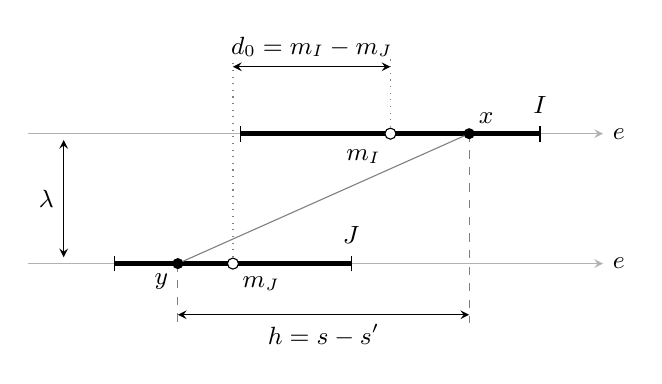
\begin{tikzpicture}[x=1cm,y=1cm,>=stealth, font=\small]
 \draw[gray!60,->] (-0.3,1.65)--(7,1.65);
 \draw[gray!60,->] (-0.3,0)--(7,0);
 \draw[line width=1.6pt] (2.4,1.65)--(6.2,1.65);
 \draw[line width=1.6pt] (0.8,0)--(3.8,0);
 \draw (2.4,1.55)--(2.4,1.75) (6.2,1.55)--(6.2,1.75);
 \draw (0.8,-0.1)--(0.8,0.1) (3.8,-0.1)--(3.8,0.1);
 \node[above] at (6.2,1.78) {$I$};
 \node[above] at (3.8,0.13) {$J$};
 \node[right] at (7,1.65) {$e$};
 \node[right] at (7,0) {$e$};
 \draw[<->] (0.15,0.08)--node[left] {$\lambda$}(0.15,1.57);
 \draw[gray,dashed] (1.6,0)--(1.6,-0.75);
 \draw[gray,dashed] (5.3,1.65)--(5.3,-0.75);
 \draw[<->] (1.6,-0.65)--node[below] {$h=s-s'$}(5.3,-0.65);
 \draw[gray] (1.6,0)--(5.3,1.65);
 \fill (5.3,1.65) circle (2pt);
 \fill (1.6,0) circle (2pt);
 \node[above right] at (5.3,1.65) {$x$};
 \node[below left] at (1.6,0) {$y$};
 \draw[gray,dotted] (2.3,0)--(2.3,2.6);
 \draw[gray,dotted] (4.3,1.65)--(4.3,2.6);
 \draw[<->] (2.3,2.5)--node[above] {$d_0=m_I-m_J$}(4.3,2.5);
 \fill[white] (4.3,1.65) circle (2pt);
 \draw (4.3,1.65) circle (2pt);
 \fill[white] (2.3,0) circle (2pt);
 \draw (2.3,0) circle (2pt);
 \node[below left] at (4.3,1.57) {$m_I$};
 \node[below right] at (2.3,-0.04) {$m_J$};
\end{tikzpicture}
\caption{The transverse separation is $\lambda$, whereas the kernel
depends on the longitudinal difference $h$.  The distribution of $h$
over $I\times J$ is symmetric about the midpoint separation $d_0$,
which need not be zero.}
\label{fig:interval-geometry}
\end{figure}

\begin{lemma}[Weighted interval comparison]\label{lem:interval-pair}
Let $n\ge3$, $\lambda>0$, and let $I,J\subset\R$ be nonempty open
intervals, possibly unbounded.  Let $c_I,c_J\ge0$, with $I$ bounded
whenever $c_I>0$ and $J$ bounded whenever $c_J>0$.  Then
\begin{equation}\label{eq:interval-pair}
\begin{split}
 \int_{I\times J}(c_I+c_J)\mathcal K\,\dd s\,\dd s'
 \le \int_{I\times J}\Bigl[
 &c_I\overline{\mathcal K}_I+c_J\overline{\mathcal K}_J\\
 &+\bigl((n-2)\min(c_I,c_J)\mathcal D
                  +|c_I-c_J|\bigr)\mathcal K\Bigr]\,\dd s\,\dd s'.
\end{split}
\end{equation}
Every term is nonnegative and the inequality is understood for extended
integrals.  An endpoint term with coefficient zero is defined to be zero,
without evaluating the endpoint average.
\end{lemma}

\begin{proof}
If at most one coefficient is positive, then
$|c_I-c_J|=c_I+c_J$, so the inequality holds pointwise before integration.
Suppose now that both coefficients are positive.  Both intervals are
bounded and $\lambda>0$, so all integrals in the following calculation
are finite.

Integration by parts in the first variable gives
\[
 \int_I(\mathcal K-\overline{\mathcal K}_I)\,\dd s
 =-\int_I(s-m_I)\partial_s\mathcal K\,\dd s.
\]
The corresponding identity in the second variable, together with
\[
 \partial_s\mathcal K=-(n-2)\frac{h}{\lambda^2+h^2}\mathcal K,
 \qquad
 \partial_{s'}\mathcal K=(n-2)\frac{h}{\lambda^2+h^2}\mathcal K,
\]
yields
\begin{equation}\label{eq:midpoint-identity}
 \int_{I\times J}
  (2\mathcal K-\overline{\mathcal K}_I-\overline{\mathcal K}_J)
   \,\dd s\,\dd s'
 =(n-2)\int_{I\times J}
    \frac{h^2-d_0h}{\lambda^2+h^2}\mathcal K\,\dd s\,\dd s'.
\end{equation}

The sign of the midpoint term follows directly from interval overlap.
If $L=|I|$ and $M=|J|$, the pushforward of $\dd s\,\dd s'$ under
$(s,s')\mapsto h=s-s'$ has density
\[
 \rho(h)=F(|h-d_0|),\qquad
 F(r)=\max\left\{0,\min\left\{L,M,\frac{L+M}{2}-r\right\}\right\}
 \quad(r\ge0).
\]
Indeed, $\rho(h)=|I\cap(J+h)|$, the overlap length of two intervals
whose centers are separated by $|h-d_0|$.
The function $F$ is nonincreasing.  If $d_0\ge0$ and $h>0$, then
$|h-d_0|\le|h+d_0|$, hence $\rho(h)\ge\rho(-h)$; for $d_0\le0$
the inequality is reversed.  Pairing positive and negative $h$ against
the odd function
$h\mathcal K(h)/(\lambda^2+h^2)$ therefore proves
\[
 d_0\int_{I\times J}\frac{h}{\lambda^2+h^2}
                 \mathcal K\,\dd s\,\dd s'\ge0.
\]
Consequently the left side of \eqref{eq:midpoint-identity} is at most
$(n-2)\int_{I\times J}\mathcal D\mathcal K$.

Multiply this last estimate by $c=\min(c_I,c_J)$.  Each individual
endpoint defect is bounded above by $\int_{I\times J}\mathcal K$,
because its subtracted endpoint average is nonnegative.  The remaining
coefficients are $c_I-c$ and $c_J-c$, whose sum is $|c_I-c_J|$.
Adding these estimates and moving the finite endpoint terms to the
right proves \eqref{eq:interval-pair}.
\end{proof}

The nonnegative formulation is essential when $n=3$: even for
$\lambda>0$, an integral of $\mathcal K$ over an unbounded partner
interval can diverge.  Lemma~\ref{lem:interval-pair} makes no subtraction
on such an interval.

\section{Pressure from weighted source layers}\label{sec:pressure}

We retain the sources, potentials, interaction measure, and cutoffs
defined above.  In particular, $n\ge3$, $A,B>-2$, $p,q>0$, and $pq>1$.
All constants in this section are uniform over admissible solution
pairs.  A subscript records permitted dependence on the auxiliary
parameters; constants are always independent of the direction $e$.

\begin{proposition}[Localized pressure]\label{prop:pressure}
Let $(u,v)$ be a positive solution pair as in Theorem~\ref{thm:main},
with $n\ge3$, $A,B>-2$, and $pq>1$.  For every $\eps>0$ there is a
constant $C_\eps$, depending only on the equation parameters and
$\eps$, such that
\begin{equation}\label{eq:pressure}
 aW_f+bW_g
 \le(n-2)\int_{\R^n\times\R^n}w(x)D(x,y)\,\dd\pi(x,y)
       +\eps E+C_\eps.
\end{equation}
\end{proposition}

The proof must accommodate the spatial factors at source-layer
endpoints.  We localize to short intervals, where those factors vary
by at most $C\delta d(x)$, and use caps of angular radius proportional
to $d(x)$.  The factor $d$ converts both errors into multiples of
$E$, by $dw\le C\eta$ from \eqref{eq:cutoff-bounds}.

\subsection{Angular localization}

Write $\mathbb E_e$ and $\mathbb P_e$ for expectation and probability
under normalized surface measure on $\Sph$.  Fix
$0<\kappa<1$ and $0<\delta<1/4$, and put
\[
 \ell(x)=\delta d(x)^m\qquad(d(x)>0).
\]
Choose a fixed nonnegative smooth function $\psi$ on $[0,\infty)$,
equal to one near zero, supported in $[0,1]$, and bounded by one.
For $0<l\le1$ and any $\theta\in\Sph$, set
\[
 Z(l)=\mathbb E_e\psi(|e-\theta|/l).
\]
Rotational invariance makes this independent of $\theta$.  Chordal
polar coordinates give
\[
 Z(l)=\frac{|\mathbb S^{n-2}|}{|\Sph|}
       l^{n-1}\int_0^1\psi(t)t^{n-2}
                  (1-l^2t^2/4)^{(n-3)/2}\,\dd t
\]
and therefore
$c l^{n-1}\le Z(l)\le C l^{n-1}$ and
$|Z'(l)|\le C l^{n-2}$.

Define the cap weight by
\begin{equation}\label{eq:cap-weight}
 h_e(x)=w(x)\frac{\psi(|e-\omega_x|/(\kappa d(x)))}{Z(\kappa d(x))}
 \quad(1<|x|<2),\qquad h_e(x)=0\quad\hbox{otherwise}.
\end{equation}
Its exact normalization is $\mathbb E_e h_e(x)=w(x)$.  Differentiation,
using \eqref{eq:cutoff-bounds}, gives
\begin{equation}\label{eq:cap-bounds}
 0\le h_e(x)\le C_\kappa d(x)^{N-n},\qquad
 |\nabla h_e(x)|\le C_\kappa d(x)^{N-n-1}
 \quad(1<|x|<2).
\end{equation}
To check the second estimate, derivatives of the cap profile cost at
most $C_\kappa/d$, and differentiation of $Z(\kappa d)^{-1}$ costs
the same relative factor.  The profile is constant near its center,
so the norm $|e-\omega_x|$ causes no differentiability problem there.
The weight extends continuously by zero across both boundary spheres:
$w$ vanishes quadratically at $|x|=1$, and $N-n>1$ at $|x|=2$.

As in Lemma~\ref{lem:localization}, call a pair close if
$|x-y|\le\ell(z)$ for at least one endpoint $z\in\{x,y\}$ with
$d(z)>0$.  On its segment, $d$ is comparable to $d(z)$ because $d$
is $1$-Lipschitz and $\ell(z)\le\delta d(z)$.  Integrating the
derivative bound across the pieces of this segment proves
\begin{equation}\label{eq:cap-oscillation}
 |h_e(x)-h_e(y)|
 \le C_\kappa\delta d(z)^{N-n-1+m}
 \le C_\kappa\delta d(z)^N,
\end{equation}
where $N-n-1+m=N+2$.  The interaction marginals bound the integral
over close pairs by $C_\kappa\delta E$.
On the complementary pairs, \eqref{eq:cap-bounds} and the tail bound
\eqref{eq:uniform} give, for example, the bound
\[
 C_\kappa\int_{B_2}f(x)d(x)^{N-n}\ell(x)^{2-n}\,\dd x
 \le C_{\kappa,\delta},
\]
since $N-n-m(n-2)=3n+8>0$; the other endpoint is identical with
$g$ in place of $f$.  We have proved
\begin{equation}\label{eq:cap-mismatch}
 \int|h_e(x)-h_e(y)|\,\dd\pi(x,y)
 \le C_\kappa\delta E+C_{\kappa,\delta}.
\end{equation}
Moreover, on the support of $h_e(x)$,
\[
 |D_e(x,y)-D(x,y)|\le2|e-\omega_x|\le2\kappa d(x).
\]
Averaging and using $dw\le C\eta$ gives
\begin{equation}\label{eq:cap-pressure}
 \mathbb E_e\int h_e(x)D_e(x,y)\,\dd\pi(x,y)
 \le\int w(x)D(x,y)\,\dd\pi(x,y)+C\kappa E.
\end{equation}
Here the constant $C$ is independent of $\kappa,\delta$.

\subsection{Measurable intervals and their loss}

For $0<t<f(x)$, let $I$ be the connected component containing $x$
of the source layer $\{f>t\}$ on the line $x+\R e$.  Assign it
the weight
\begin{equation}\label{eq:component-weight}
 \chi_I=
 \begin{cases}
  \displaystyle\inf_I h_e,
   &I\text{ bounded and }|I|\le2\delta\inf_I d,\\
  0,&\text{otherwise}.
 \end{cases}
\end{equation}
Set $\chi_f(e,x,t)=\chi_I$.  Define $\chi_g(e,y,t')=\chi_J$
in the same way from $\{g>t'\}$.  In particular,
$0\le\chi_f(e,x,t)\le h_e(x)$ and
$0\le\chi_g(e,y,t')\le h_e(y)$.

All these functions, as well as finite endpoints, are jointly
measurable.  Indeed, with the convention $f(0)=0$, the set
$\{(x,t):x\ne0,\ 0<t<f(x)\}$ is open.  The forward exit distance
of its line component exceeds $r\ge0$ exactly when the compact
segment $\{x+se:0\le s\le r\}$ is contained in the layer.  This
is an open condition in $(e,x,t)$; the backward exit distance is
treated in the same way.  Their sum, including the value $+\infty$,
is the measurable component length.  The infima in
\eqref{eq:component-weight} can be taken over rational offsets
between these two exits, since $d$ and $h_e$ are continuous.
This proves the assertion, including measurability in $e$, without
a choice of coordinates on the varying spaces $e^\perp$.

For each direction define the nonnegative losses
\begin{align*}
 L_f(e)&=\int_{\R^n}u(x)\int_0^{f(x)}
                 (h_e(x)-\chi_f(e,x,t))\,\dd t\,\dd x,\\
 L_g(e)&=\int_{\R^n}v(y)\int_0^{g(y)}
                 (h_e(y)-\chi_g(e,y,t'))\,\dd t'\,\dd y.
\end{align*}
They are finite for each fixed solution and direction, since $h_e$
is bounded and supported on the compact annulus $1\le|x|\le2$.
This finiteness does not assert a uniform bound on those marginals.

\begin{lemma}[Averaged layer loss]\label{lem:layer-loss}
For the cap weights \eqref{eq:cap-weight} and component weights
\eqref{eq:component-weight}, under the hypotheses of
Proposition~\ref{prop:pressure}, every $P\ge1$ satisfies
\begin{equation}\label{eq:layer-loss}
 \mathbb E_e\bigl(L_f(e)+L_g(e)\bigr)
 \le\bigl(C_\kappa\delta+C_{\kappa,\delta}P^{-1}\bigr)E+CP.
\end{equation}
The constants in the relative coefficient are independent of $P$,
and the last constant is independent of $\kappa,\delta,P$.
\end{lemma}

\begin{proof}
We prove the assertion for $f,u$; the same argument applies to $g,v$.
Only $1<|x|<2$ contributes.  Fix such an $x$ and write $d=d(x)$
and $\ell=\delta d^m$.
If the component $I$ at level $t$ has $|I|\le\ell$, then
\[
 \inf_I d\ge d-\ell\ge(1-\delta)d,
 \qquad |I|\le\delta d\le2\delta\inf_I d.
\]
It therefore passes the length condition in
\eqref{eq:component-weight}.  Estimate~\eqref{eq:cap-oscillation}
shows that its entire loss of weight is at most
$C_\kappa\delta d^N$.

If $|I|>\ell$, at least one of its two portions from $x$ contains
a segment of length $\ell/2$.  Let $F$ be the set of directions
whose forward segment of that length lies in $\{f>t\}$.  Polar
integration centered at $x$ gives
\[
 \int_{B_{\ell/2}(x)}f
 \ge \frac{|\Sph|}{n}\,t(\ell/2)^n\mathbb P_e(F).
\]
The long-interval event is contained in $F\cup(-F)$.  Antipodal
symmetry, followed by the source bound in \eqref{eq:uniform}, yields
\begin{equation}\label{eq:long-interval}
 \mathbb P_e\{|I|>\ell\}
 \le \frac{C}{t\ell^n}\int_{B_\ell(x)}f
 \le\frac{C}{t\ell^n}.
\end{equation}
Here $B_\ell(x)\subset B_4$; only its containment in a fixed
centered ball is used.

For $t\ge P d^{-k}$, the expected loss on long intervals is bounded
using the supremum of $h_e(x)$ times the probability in
\eqref{eq:long-interval}.  No independence is needed.  The result is
\[
 C_\kappa d^{N-n}\,C\delta^{-n}P^{-1}d^{k-mn}
   =C_{\kappa,\delta}P^{-1}d^N,
\]
because $k=n(m+1)$.  Integrating the short- and long-interval
estimates over these high levels, and then against $u(x)\,\dd x$,
gives at most
$\bigl(C_\kappa\delta+C_{\kappa,\delta}P^{-1}\bigr)E_f$.

For the remaining levels use the exact cap normalization:
\[
 \int_0^{\min\{f(x),Pd^{-k}\}}
        \mathbb E_e(h_e(x)-\chi_f(e,x,t))\,\dd t
 \le Pd^{-k}w(x)\le CPd^{N-1-k}\le CP.
\]
The last exponent equals $n+1$.  Integration against $u$ is bounded
by $CP$ by \eqref{eq:uniform}.  Repeating the proof for $g,v$
proves \eqref{eq:layer-loss}.
\end{proof}

\subsection{Weighted endpoints and nonnegative integration}

Suppose $\chi_I>0$ for an $f$-layer at level $t$.  Then $I$ is
bounded and $h_e\ge\chi_I>0$ on it.  Continuity gives the same
inequality at its two endpoints $x_-,x_+$, so they lie in the
annulus $1<|x|<2$.  Continuity of $f$ there and maximality of the
component imply
\[
 f(x_-)=f(x_+)=t,\qquad
 u(x_\pm)=t^{1/q}|x_\pm|^{-B/q}.
\]
For any $x\in I$, \eqref{eq:component-weight} gives
$|x_\pm-x|\le2\delta d(x)$.  The positive radial function
$|x|^{-B/q}$ has a bounded relative Lipschitz constant on
$1\le|x|\le2$.  Thus, with
$\overline u_I=(u(x_-)+u(x_+))/2$, we have
\begin{equation}\label{eq:weighted-endpoints}
 \left|\overline u_I-(t/|x|^B)^{1/q}\right|
 \le C\delta d(x)(t/|x|^B)^{1/q}
 \le C\delta d(x)u(x).
\end{equation}
The same statement holds for a positive-weight $g$-component $J$,
with endpoint average $\overline v_J$ and ideal value
$(t'/|y|^A)^{1/p}$.  When a component weight is zero, every product
involving its endpoint average is defined as zero without selecting
or evaluating endpoints.

Fix a direction $e$ and levels $t,t'>0$.  On two distinct parallel
lines $x=z+se$ and $y=z'+s'e$, apply
Lemma~\ref{lem:interval-pair} to each pair of layer components $I,J$
with $c_I=\chi_I$ and $c_J=\chi_J$.  Since
$\min(\chi_I,\chi_J)\le h_e(x)$, it gives
\begin{equation}\label{eq:layer-pair}
\begin{split}
 \int_{I\times J}(\chi_I+\chi_J)\mathcal K
 \le\int_{I\times J}\Bigl[
  &\chi_I\overline{\mathcal K}_I+\chi_J\overline{\mathcal K}_J\\
  &+\bigl((n-2)h_e(x)D_e(x,y)+|\chi_I-\chi_J|\bigr)
       \mathcal K\Bigr],
\end{split}
\end{equation}
where the measures are $\dd s\,\dd s'$.  At this stage all terms
are nonnegative extended integrals.

Each open line layer has at most countably many components.  Sum
\eqref{eq:layer-pair} over the two sets of components, and integrate
in $z,z'\in e^\perp$ and $t,t'>0$.  The summed functions are the
jointly measurable functions described above; hence Tonelli's
Theorem applies.  The coincident-line set $z=z'$ is null and may be
omitted.  By the potential identities \eqref{eq:potentials}, the two
terms on the left become
\begin{align*}
 U_f(e)&=\int\int_0^{f(x)}\chi_f(e,x,t)u(x)\,\dd t\,\dd x,\\
 U_g(e)&=\int\int_0^{g(y)}\chi_g(e,y,t')v(y)\,\dd t'\,\dd y.
\end{align*}
Similarly, the endpoint terms become
\begin{align*}
 V_f(e)&=\int\int_0^{f(x)}\chi_f(e,x,t)\overline u_I\,\dd t\,\dd x,\\
 V_g(e)&=\int\int_0^{g(y)}\chi_g(e,y,t')\overline v_J\,\dd t'\,\dd y.
\end{align*}
For example, integrating $\overline{\mathcal K}_I$ over all
$(y,t')$ layers recovers the average of $K*g$ at $x_-,x_+$.
For each selected endpoint the omitted $y$-points comprise one
affine line, which is Lebesgue null in $\R^n$, so the recovered
potential is exactly $\overline u_I$.

We now verify finiteness before any subtraction.  Set
\[
 H_f(e)=\int h_e(x)f(x)u(x)\,\dd x,
 \qquad H_g(e)=\int h_e(y)g(y)v(y)\,\dd y.
\]
Both are finite for every fixed solution and direction because the
cap weights are bounded and supported on a compact annulus.
We have $U_f\le H_f$, $U_g\le H_g$, while
\eqref{eq:weighted-endpoints} gives $V_f\le C H_f$ and
$V_g\le C H_g$.  The integrated pressure term is at most
$(n-2)H_f$.  Finally,
\[
 |\chi_f(e,x,t)-\chi_g(e,y,t')|\le h_e(x)+h_e(y),
\]
so its integrated contribution is at most $H_f+H_g$, again by
Tonelli and the two potential marginals.  All the integrated terms
are therefore finite, even when $n=3$.  In particular, we have
never subtracted the possibly infinite integrals over an unbounded
line component.

It is now legitimate to subtract $V_f+V_g$.  The sharper mismatch
bound
\begin{align*}
 |\chi_f(e,x,t)-\chi_g(e,y,t')|
 \le{}&|h_e(x)-h_e(y)|\\
      &+(h_e(x)-\chi_f(e,x,t))
        +(h_e(y)-\chi_g(e,y,t'))
\end{align*}
shows that the resulting finite quantity
\[
\begin{split}
 S_e={}&\int\int_0^{f(x)}\chi_f(e,x,t)(u(x)-\overline u_I)\,\dd t\,\dd x\\
   &+\int\int_0^{g(y)}\chi_g(e,y,t')(v(y)-\overline v_J)\,\dd t'\,\dd y
\end{split}
\]
satisfies
\begin{equation}\label{eq:integrated-pressure}
 S_e\le(n-2)\int h_e(x)D_e(x,y)\,\dd\pi(x,y)
       +\int|h_e(x)-h_e(y)|\,\dd\pi(x,y)+L_f(e)+L_g(e).
\end{equation}
The quantity $S_e$ need not be nonnegative; only the preceding
unsubtracted expressions were treated with Tonelli's Theorem.

\subsection{Recovery of the cutoff pressure}

The exact weighted layer identity is
\begin{equation}\label{eq:weighted-layer-identity}
 \int_0^{f(x)}\left[u(x)-(t/|x|^B)^{1/q}\right]\,\dd t
 =\frac{f(x)u(x)}{q+1}=a f(x)u(x)\qquad(x\ne0).
\end{equation}
Indeed, the integral of $(t/|x|^B)^{1/q}$ equals
$qf(x)u(x)/(q+1)$.  The analogous identity for $g$ has coefficient
$b=1/(p+1)$.
To compare \eqref{eq:weighted-layer-identity} with $S_e$, set
$\tau=(t/|x|^B)^{1/q}$.  Since $0\le\tau\le u(x)$,
\begin{align*}
 &h_e(x)(u(x)-\tau)-\chi_f(e,x,t)(u(x)-\overline u_I)\\
 &\quad=(h_e(x)-\chi_f(e,x,t))(u(x)-\tau)
                  +\chi_f(e,x,t)(\overline u_I-\tau)\\
 &\quad\le(h_e(x)-\chi_f(e,x,t))u(x)
                  +C\delta d(x)h_e(x)u(x),
\end{align*}
by \eqref{eq:weighted-endpoints}; the zero-weight case has the same
bound under the convention already stated.  Integrating and treating
the $g$-layer in the same way gives
\begin{equation}\label{eq:pressure-recovery}
\begin{split}
 aH_f(e)+bH_g(e)
 \le{}&S_e+L_f(e)+L_g(e)\\
       &+C\delta\int d(x)h_e(x)f(x)u(x)\,\dd x\\
       &+C\delta\int d(y)h_e(y)g(y)v(y)\,\dd y.
\end{split}
\end{equation}

\begin{proof}[Proof of Proposition~\ref{prop:pressure}]
Combine \eqref{eq:integrated-pressure} and
\eqref{eq:pressure-recovery}, and average over $e$.  This incurs
two copies of $L_f+L_g$.  The identities
$\mathbb E_e h_e=w$ and $dw\le C\eta$, together with
\eqref{eq:cap-mismatch}, \eqref{eq:cap-pressure}, and
Lemma~\ref{lem:layer-loss}, give
\[
\begin{split}
 aW_f+bW_g\le{}&(n-2)\int w(x)D(x,y)\,\dd\pi(x,y)\\
 &+\bigl(C\kappa+C_\kappa\delta
                    +C_{\kappa,\delta}P^{-1}\bigr)E
   +C_{\kappa,\delta,P}.
\end{split}
\]
The constant multiplying $\kappa$ is independent of all three
auxiliary parameters; the one multiplying $\delta$ is independent
of $\delta,P$; and the one multiplying $P^{-1}$ is independent of
$P$.  First choose $\kappa$ sufficiently small, next $\delta$
sufficiently small, and finally $P$ sufficiently large, so that
the relative coefficient is at most $\eps$.  The remaining
additive constant is finite and uniform over the solution pair.
This proves \eqref{eq:pressure}.
\end{proof}

\section{The energy bound and the scaling contradiction}
\label{sec:conclusion}

We now close the argument. Throughout this section the reductions of
Section~\ref{sec:preliminaries} have been made, so
\(n\ge3\), \(A,B>-2\), \(pq>1\), and the gap
\(\gamma\) in Equation~\eqref{eq:gap} is positive.

\begin{proposition}[Uniform local energy bound]\label{prop:energy}
For the fixed equation parameters there is a constant \(C\), independent
of the solution pair, such that
\begin{equation}\label{eq:energy-bound}
 \int_{B_1}\bigl(|x|^B u^{q+1}+|x|^A v^{p+1}\bigr)\dd x
 \le E\le C.
\end{equation}
\end{proposition}

\begin{proof}
Write
\[
 T=\int w(x)D(x,y)\dd\pi(x,y),\qquad
 Q=\int\bigl(\Phi(x,y)-\eta(x)+w(x)D(x,y)\bigr)\dd\pi(x,y).
\]
Lemma~\ref{lem:localization} gives, for every \(\eps>0\),
\begin{equation}\label{eq:closing-errors}
 |Q|+|E_f-E_g|\le\eps E+C_\eps.
\end{equation}
The virial identity, Equation~\eqref{eq:virial}, is therefore exactly
\begin{equation}\label{eq:closing-identity}
\begin{gathered}
 c_1E_f+c_2E_g
   =aW_f+bW_g-(n-2)T+(n-2)Q,\\
 c_1=a(n+B)-(n-2),\quad c_2=b(n+A).
\end{gathered}
\end{equation}
Proposition~\ref{prop:pressure} bounds the first three terms on the
right from above by \(\eps E+C_\eps\). Consequently
\[
 c_1E_f+c_2E_g\le(n-1)\eps E+C_\eps.
\]
Here and below the additive constant may change, but remains independent
of the solution. Since \(c_1+c_2=\gamma\),
\[
 c_1E_f+c_2E_g
   =\frac{\gamma}{2}E+\frac{c_1-c_2}{2}(E_f-E_g).
\]
Using Equation~\eqref{eq:closing-errors}, we obtain
\[
 \frac{\gamma}{2}E
 \le\left(n-1+\frac{|c_1-c_2|}{2}\right)\eps E+C_\eps.
\]
Choose \(\eps\) so that the coefficient of \(E\) on the right is at
most \(\gamma/4\). This proves the universal bound on \(E\).
The first inequality in Equation~\eqref{eq:energy-bound} follows from
\(\eta=1\) on \(B_1\) and the nonnegativity of the energy densities.
\end{proof}

\begin{proof}[Proof of Theorem~\ref{thm:main}]
The elementary reductions in Section~\ref{sec:preliminaries} already
exclude \(n=2\), weights at most \(-2\), and \(pq\le1\).
Suppose a solution exists in the remaining range. For every \(R>0\),
the pair
\[
 u_R(x)=R^\alpha u(Rx),\qquad v_R(x)=R^\beta v(Rx)
\]
is an admissible solution with the same equation parameters.
Proposition~\ref{prop:energy} applies to every such pair with the same
constant. Both energy terms have the same dilation exponent:
\begin{align*}
 &\int_{B_1}
   \bigl(|x|^B u_R(x)^{q+1}+|x|^A v_R(x)^{p+1}\bigr)\dd x\\
 &\hspace{2em}
 =R^{\alpha+\beta+2-n}
   \int_{B_R}\bigl(|x|^B u(x)^{q+1}+|x|^A v(x)^{p+1}\bigr)\dd x.
\end{align*}
For \(R\ge1\), the last integral is at least its fixed, strictly
positive value on \(B_1\). It is finite on every bounded ball.
Equation~\eqref{eq:gap} and \(1-a-b>0\) give
\(\alpha+\beta+2-n>0\), so the displayed expression tends to
infinity as \(R\to\infty\). This contradicts the uniform bound.
\end{proof}

\begin{corollary}[H\'enon--Lane--Emden classification; Phan's Conjecture C]
\label{cor:phan-classification}
Let \(n\ge3\) be an integer, let \(p,q>0\), and let \(A,B>-2\).
There is no pair
\[
 u,v\in C^2(\R^n\setminus\{0\})\cap C(\R^n),
 \qquad u(x)>0,\quad v(x)>0\quad(x\in\R^n),
\]
satisfying Equation~\eqref{eq:system} at every \(x\ne0\) if and only if
\[
 \frac{n+A}{p+1}+\frac{n+B}{q+1}>n-2.
\]
When the reverse weak inequality holds, such a pair exists and can be
chosen radial.
\end{corollary}

\begin{proof}
The strict inequality gives nonexistence by Theorem~\ref{thm:main}.
Suppose instead that
\[
 \frac{n+A}{p+1}+\frac{n+B}{q+1}\le n-2.
\]
Since \(n+A,n+B>n-2>0\),
\[
 \frac1{p+1}+\frac1{q+1}
 <\frac1{n-2}\left(\frac{n+A}{p+1}+\frac{n+B}{q+1}\right)
 \le1.
\]
Thus \(pq>1\), because
\(1-1/(p+1)-1/(q+1)=(pq-1)/((p+1)(q+1))\).

We now apply Proposition~B of Phan~\cite{Phan}, which states the radial
ground-state theorem of Bidaut-V\'eron and
Giacomini~\cite[Theorem~1.4(i)]{BidautVeronGiacomini2010} for the same
equation and solution class, with \(n\ge3\), \(A,B>-2\), and \(p,q>0\).
Its radial existence region is exactly the displayed reverse weak
inequality, including equality on the critical hyperbola. In the original
Hamiltonian notation, the substitution is \(N=n\), \(a=A\), \(b=B\),
\(\delta=p\), and \(\mu=q\), with both differential-operator exponents
equal to \(2\); the preceding calculation verifies the standing
superlinearity condition \(D=\delta\mu-1>0\).

The original ground states have positive radial profiles \(U,V\) on
\((0,\infty)\), classical there and continuous at zero. This origin
regularity gives the strict positivity at zero required here: the radial
equation makes
\(r^{n-1}U'(r)\) strictly decreasing. Its limit as \(r\downarrow0\)
must be zero: a nonzero or infinite limit would contradict continuity
of \(U\) at zero after integration against \(r^{1-n}\). Hence
\(U'(r)<0\), and \(U(0)\ge U(r)>0\) for every \(r>0\). The same
argument applies to \(V\). Thus \(u(x)=U(|x|)\) and
\(v(x)=V(|x|)\) belong to the stated solution class and are strictly
positive on all of \(\R^n\). Radial existence in this class rules out
unrestricted nonexistence under the reverse weak inequality, completing
the equivalence.
\end{proof}

This classification is a consequence of Theorem~\ref{thm:main} joined
to the cited radial existence theorem, rather than a new construction
of ground states. The complementary existence assertion is restricted
to \(n\ge3\) and \(A,B>-2\); the broader nonexistence statement of
Theorem~\ref{thm:main} is unchanged.

\bibliographystyle{plain}
\bibliography{references}
\end{document}
